%!TEX root = ../dissertation.tex

\chapter{Implementation}
\label{implementation}

As a reminder, the coordinate system convention that will be used throughout this chapter is the computer vision one mentioned in section \ref{cha2:represent}. 

\section{Flow Overview}
\begin{figure}[ht]
	\centering
	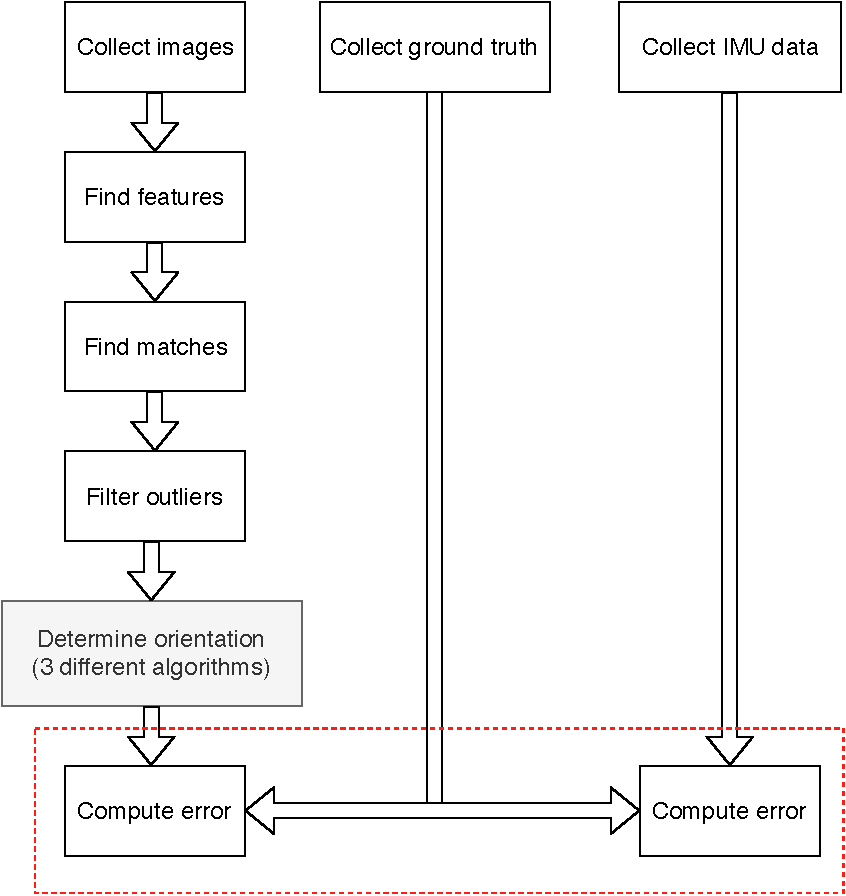
\includegraphics[width=0.7\textwidth]{images/approach.pdf}
	\caption[Flow Diagram]{Flow Diagram. Using the \acrshort{rgb} camera, two images are collected, before and after rotation. In each image, features are detected and matched between them. Some matches might be false or have too much noise, so they are filtered out. Using the matches information, the executed rotation is determined using an estimation algorithm. 3 algorithms will be put to test. Finally, the rotation determined is compared against the ground truth. The \acrshort{imu}'s orientation output is also compared against the ground truth to evaluate the improvement in relation to the camera.}
	\label{cha3:methodology:approach}
\end{figure}
Figure \ref{cha3:methodology:approach} shows the flow of the procedures that accompany the determination of the eye rotation. Firstly two images are collected, before and after rotating. In each of the images, points that make the image unique and identifiable, called feature points, are detected. These points are then matched together between the images. Because some may be wrongly matched, as mentioned on section \ref{cha2:robustest}, they need to go through a filtering process. Afterwards, the rotation can be determined using one the algorithms presented on section \ref{methods}. In order, to understand which one is best they are all put to test by determining their error against the ground truth. Besides that, the \acrshort{imu} data is collected to compare its performance against the camera.\\

This workflow is what is necessary to determine the rotation of the camera under real data sets. However, in order to evaluate the three algorithms in a controlled environment, a simulator was implemented and what it does is generate image points matches with defined rotations. This points may have added non-gaussian noise, or even false matches to test the performance of the outlier filtering. 

Both the simulator and the procedures to deal with real data were implemented in Matlab \footnote{\href{https://www.mathworks.com/products/matlab.html}{https://www.mathworks.com/products/matlab.html}} and can be found in the this thesis github repository\footnote{\href{https://github.com/Mrrvm/Orient/tree/master/Matlab}{https://github.com/Mrrvm/Orient/tree/master/Matlab}}. A C++ library was also created to deal with the data on the real system for convenience and computation speed, and can also be found at the repository\footnote{\href{https://github.com/Mrrvm/Orient/tree/master/C++}{https://github.com/Mrrvm/Orient/tree/master/C++}}.

\section{Simulator}

To generate corresponding points in two simulated images, first it's necessary to pick the rotation amplitude between them. This was defined as an uniform distribution between a certain lower/upper limit, so that the quantity of error obtained according to the amplitude can be tested.

\begin{minipage}{0.5\textwidth}
	\centering
	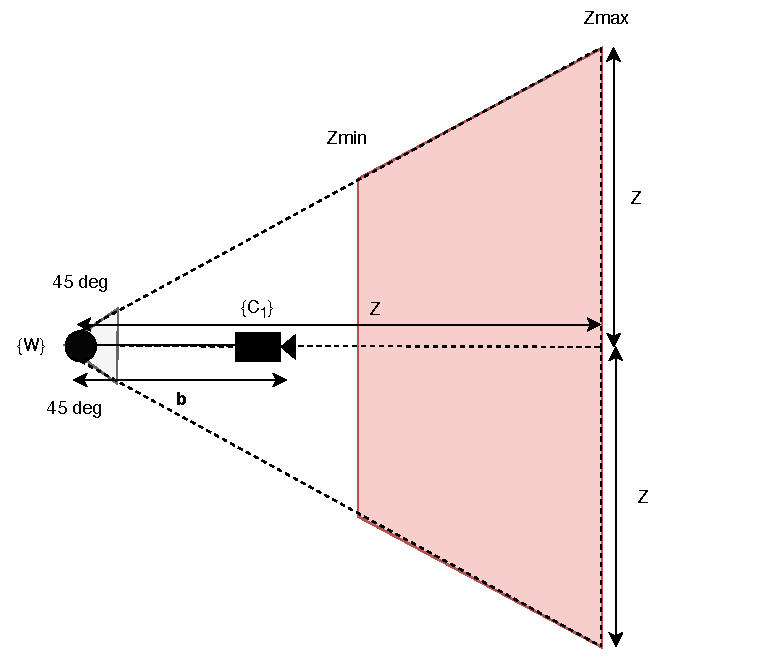
\includegraphics[width=0.9\textwidth]{images/rangesim.pdf}
	\captionof{figure}{Range in which simulated points are generated}
	\label{cha4:sec3:rangesim}
\end{minipage}
\begin{minipage}{0.5\textwidth}
	\centering
	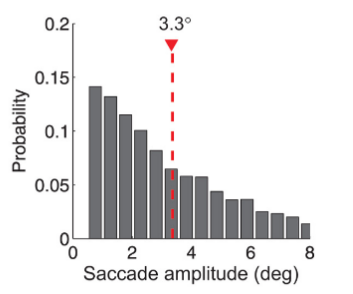
\includegraphics[width=0.6\textwidth]{images/freeview.png}
	\captionof{figure}{Probability of executing a specific \gls{saccade} amplitude when free viewing \cite{saccadeamp}}
	\label{cha4:sec3:freeview}
\end{minipage}

Afterwards, 3D points represented in the world reference frame, ${W}$, are generated within a camera viewing range of $90 \ degrees$, as represented on figure \ref{cha4:sec3:rangesim} in both $Y$ and $X$ directions, and within a range of depth $Zmin$ and $Zmax$, in order to represent a real environment where objects are at certain distances, that may affect the accuracy of the estimation. This is enough range to simulate the environment in, because the real eye moves in small saccade amplitudes. Poletti, M. et al \cite{saccadeamp}, provides information on the probability of specific \gls{saccade} amplitudes when free viewing. Free viewing is measured during normal examination of a scene, the observers freely view pictures of natural scenes, each presented for $10 \ s$. The mean of the distribution is $3.3 \ degrees$, shown on figure \ref{cha4:sec3:freeview}.

Having the points in the world frame, they are then represented in the camera reference frame before rotating, ${C_1}$, and after rotating, ${C_2}$, according to the amplitude designated between them. Finally, the 3D points are projected into the 2D image plane, and it's verified if they fit the image dimensions chosen for the simulated images.

It's possible to input Gaussian noise and also false matches into the system. For the former, random values defined in a Gaussian distribution, with a chosen variance for the simulation, are added randomly to one of the images, image before or after rotating. In the case of false matches, they are set according to the quantity chosen for the simulation, and defined as a random 2D coordinate within the image dimensions that will replace an existing correct coordinate in a random match in one of the images.

The 2D point matches are now ready to be sent to the rotation estimator.

\section{Real system}

\subsection{Setup}
\begin{figure}[ht]
	\centering
	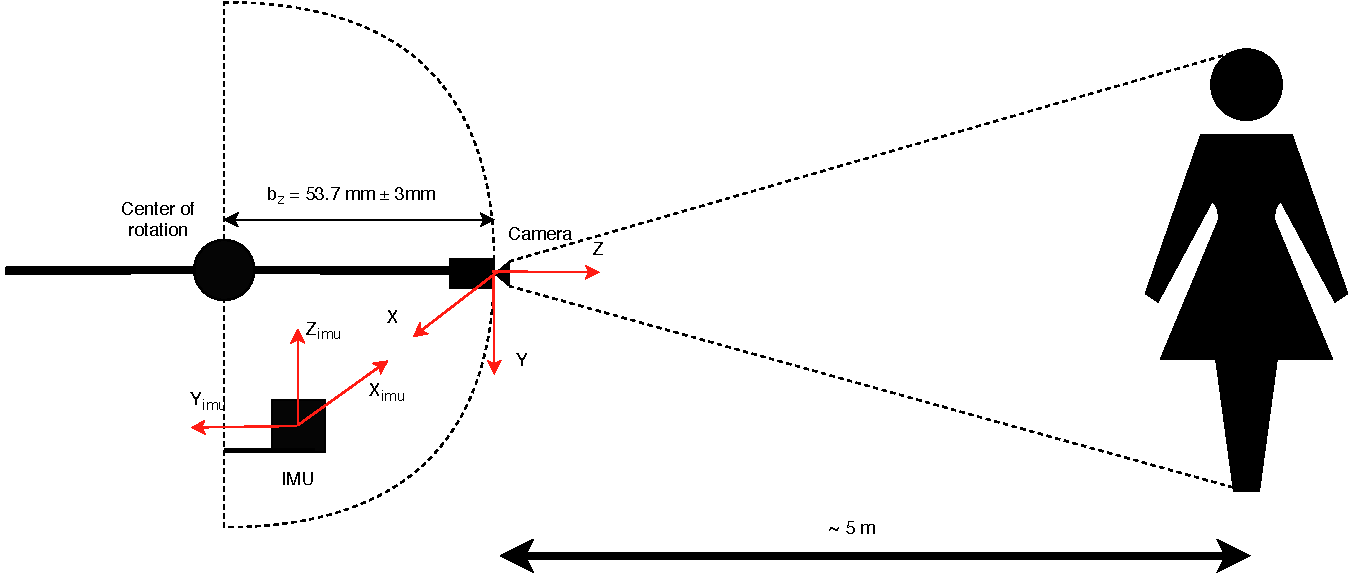
\includegraphics[width=\textwidth]{images/eyescheme.pdf}
	\caption[Eye prototype scheme used on the experiments]{Eye prototype scheme used on the experiments.}
	\label{cha4:sec3:eyescheme}
\end{figure}

\subsection{Collect images}
The images are collected using an uEye LE USB3 camera\footnote{See appendix \ref{appendix:cha2:camera} for camera specifications.} in grayscale before and after a certain rotation.

\subsection{Collect ground truth}

	Using the same camera in the same positions, the two images are taken but positioning a chessboard \footnote{See appendix \ref{appendix:cha2:chessboard} for chessboard specifications.} on the scenery, which is used to determine the ground truth through its regular pattern. The ground truth will then be utilized to evaluate the estimation algorithms performance and also the \acrshort{imu}'s performance over the camera.\\
		On Figure \ref{cha3:methodology:imagesex}, an example of the two image pairs that are collected can be observed.
	
\begin{figure}[ht]
	\centering
	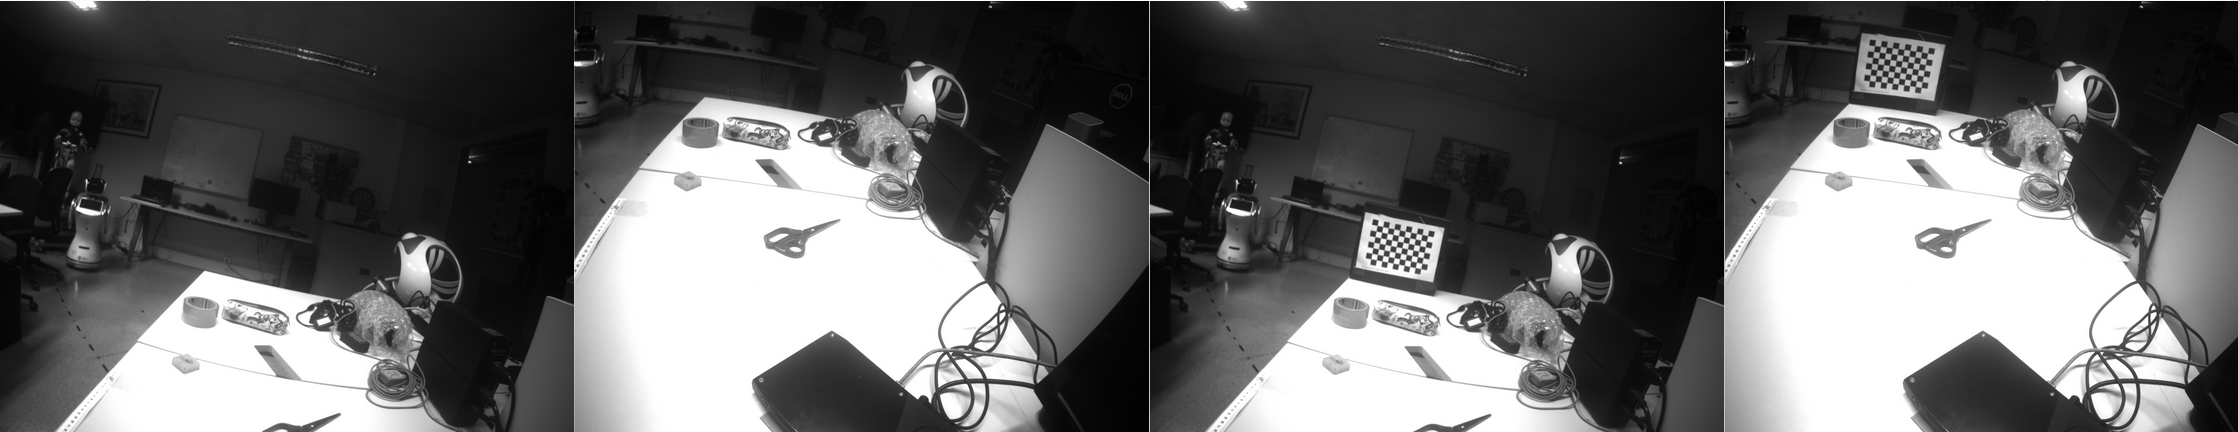
\includegraphics[width=\textwidth]{images/imagesex.png}
	\caption[Example of the two pairs of images]{Example of the two pairs of images. The first and second images are used for finding feature matches and estimating the orientation. The third and fourth images are the same as the first and second ones, respectively, but with a chessboard positioned on the scenery, and serve as ground truth to evaluate the algorithms and the \acrshort{imu}'s performance.}
	\label{cha3:methodology:imagesex}
\end{figure}

\subsection{Feature detection, matching and filtering}
\label{cha3:features}

As stated on section \ref{cha2:features} of the previous chapter,
\acrshort{sift} and \acrshort{surf} seemed to be the most promising algorithms to detect features on the collected images. Because \acrshort{surf} is faster and more accessible due to patenting concerns regarding \acrshort{sift}, it will be be used on this work.
\acrshort{flann} also previously referred to in the state of the art will be used for matching the features gathered between the two images, originating a set of point matches. The set of $n$ points matches are the pixel coordinates in the first and the second image, $\mathbf{m_{1i}} = [u_{1i} \ v_{1i}]$ and $\mathbf{m_{2i}} = [u_{2i} \ v_{2i}]$, respectively, where $i=1,...,n$.

As explained before on section \ref{cha1:problemdef}, it is necessary to gather corresponding features in consecutive images taken before and after a rotation, and to use an algorithm to estimate the orientation using those features. The latter, also referred to as keypoints or interest points, are spatial locations of an image that "stand out", allowing it to be identifiable. This points should be such that even after rotating, translating, shrinking or distorting the image, they can be found.

It is absolutely needed to have a solid detection and trust-worthy correspondence of image features (matching) when doing an "eye" movement to eventually estimate the its current orientation. Two main approaches exist to the problem of feature detection and matching. The first method finds features in one image and matches these features in the other image. The second method, which is more suitable for points in the near space, independently detects features in both images and subsequently matches them on the basis of local correspondences.

It might not be appropriate to extract features from an image having high detail (i.e. high spatial bandwidth) on the finest stable scale possible, because when matching features with another image at a different (coarser) scale those details may no longer be detectable. Therefore, it's important to extract features at a variety of scales to ensure their invariance. 

Besides scale, preserving rotation and orientation invariance is also a concern. One way to deal with this problem is to define a descriptor. This is a scaled and oriented patch around the chosen point with the local orientation and scale, from which the dominant orientation can be extracted to guarantee its invariance. \cite{multiview}

There exist a number of algorithms that can do the job. However, none of these algorithms is optimal for all images, as each of them is optimized for particular computer vision applications, with performance depending heavily on the environmental properties (illumination, image quality, contrast, ...). A comprehensive survey on the state of the art of feature detection and description  \cite{featsift} (by Salahat E. and Qasaimeh M. in 2017), proposes that ideal features should have the following properties:
\begin{itemize}
	\item Distinctiveness: the gradient variations surrounding the point should be sufficiently large;
	\item Locality: to avoid obstruction and deformation between the two images.
	\item Quantity: enough features to describe the content;
	\item Accuracy: features should be accurate enough to be detected independently of image scale, shape or pixel location;
	\item Efficiency: be detected fast enough for real-time systems;
	\item Repeatability: a high percentage of features should be detected in both images on the overlapping regions;
	\item Invariance: deformative effects on the features, due to scaling, rotation or translation are minimized;
	\item Robustness: features should be less sensitive to deformations due to noise, blur, compression, and so on.
\end{itemize} 
The review paper also presents an overview on the recent algorithms proposed on this matter, comparing them in terms of the metrics defined above. The analysis in that article suggests that Maximally stable extremal regions (MSER) and \acrfull{sift} algorithms enhance performance on computational complexity, accuracy and execution time. From the scale and rotation invariant algorithms, \acrfull{surf}, proved to be faster than \acrshort{sift}, although not as robust.

MSER (by Matas J. et al in 2002)\footnote{J. Matas J., O. Chum, M. Urban and T. Pajdla, “Robust Wide Baseline Stereo from Maximally Stable Extremal Regions,” 2002.} are areas of uniform intensity outlined by contrasting backgrounds. They are constructed by trying multiple thresholds on the input image. The ones that remain unchanged in shape over the range of thresholds are the potential features to be selected as areas of interest. The centroids of these areas can subsequently be used to create a feature descriptor for the matching step.

\acrshort{sift} (by Lowe, David G. et al in 2004) \cite{sift} algorithm detects image features using a Gaussian filter by generating increasingly blurred images, and subtracting each image to each other. This is done in several scales in order to provide scale invariance. Afterwards, a descriptor for each feature at a certain scale is created and includes information about the orientation and gradient magnitude around the point, which also grants rotation invariance.

\acrshort{surf} (by Bay, Herbert et al in 1999) \cite{surf} uses an integral image, which is an intermediate representation of the original image where the value of a location is the sum of all pixels of a rectangular region formed around that location. This is called box filter and serves as an approximation to the \gls{gauss}, speeding up the process in relation to \acrshort{sift}.

A more comprehensive explanation on both SIFT and SURF can be found at appendix \ref{appendix:cha1:sift} and \ref{appendix:cha1:surf}, respectively. Any of these 3 algorithms mentioned seems promising to use as feature detector in this work.

\subsection{Matching step}
Regarding the matching of feature descriptors, one of the most common search algorithms used is the Nearest Neighbor Search. \acrfull{flann}  \cite{flann} provides a library for performing this kind of searches in high-dimensional spaces. It contains a collection of algorithms that the authors found to  work best for nearest neighbor search and a system for automatically choosing the best algorithm and optimum parameters depending on the dataset.

\subsection{Filtering matches}

\section{Collect IMU data}
The \acrlong{imu} \footnote{See appendix \ref{appendix:cha2:imu} for \acrshort{imu} specifications.} obtains two quaternions (see section \ref{cha2:represent:quat}) with the current camera's orientation before and after rotating.

\subsection{Determine the rotation}
talk about fminsearch

\subsection{Compute the error}

\subsection{C++ Library}


